\documentclass[11pt,letterpaper]{article}
\usepackage[utf8]{inputenc}
\usepackage[english]{babel}
\usepackage{amsmath}
\usepackage{amsfonts}
\usepackage{amssymb}
\usepackage{fullpage}
\usepackage{todonotes}
\usepackage[hidelinks]{hyperref}
\usepackage{amsthm}


\newtheorem{lemma}{Lemma}
\newtheorem{theorem}{Theorem}
\newtheorem{claim}{Claim}


\newcommand{\lef}{\texttt{left}}
\newcommand{\righ}{\texttt{right}}
\newcommand{\gap}{\texttt{gap}}
\newcommand{\num}{\texttt{num}}
\newcommand{\out}{\texttt{out}}
\newcommand{\tup}{\texttt{tup}}

\newcommand{\mmin}{\texttt{MIN}}
\newcommand{\mmax}{\texttt{MAX}}
\newcommand{\var}{\texttt{Var}}

\begin{document}
\sloppy
\author{}
\title{Computing Dense Linear Operators by Linear Size Circuits: Commutativity is Essential}
\maketitle


\begin{abstract}
\todo[inline]{AM: I don't think we should put Range Queries at the front of the
paper. I think this distracts from the two main points that we'd like to make:
(i) dense/boring matrices are as ``easy'' as sparse matrices, and
(ii) commutativity is central to obtaining linear constructions. We could still
mention in the abstract that in non-commutative settings the problems that we
are solving become equivalent to classic Range Queries, from which we derive
the superlinear lower bound.~--- AK: I do agree. Adjusted the title.}

We revisit the classical problem of computing range queries over a semigroup and
its natural special case~--~computing a dense linear operator. We are interested
in the minimum number of semigroup operations needed to answer all the queries.
For commutative semigroups, we show that the special case is strictly easier:
while for range queries a~superlinear lower bound is known, a dense linear
operator can be computed by linear size circuits. We then study the role of
commutativity in these problems: it turns out to be unimportant for range
queries, but crucial for dense operators. Moreover, without commutativity both
problems are equivalent. To highlight potential applications of the presented
linear size constructions, we show how they can be used to (i) obtain linear
size representations of dense graphs, and (ii) multiply dense $n\times n$
matrices over an arbitrary commutative semiring in $O(n^2)$ time.
\end{abstract}

\tableofcontents

\section{Range Queries}
\subsection{Problem Statement}
{\em Range queries} is a~classical problem in data structures and algorithms. For a~fixed semigroup with operation~$\circ$, one is given a~sequence $x_1, x_2, \dotsc, x_n$ of semigroup elements. Then, a~range query is specified by two indices $(l,r)$ such that $1 \le l \le r \le n$. The answer to such a~query is the result of applying the semigroup operation to the corresponding range, i.e., $x_l \circ x_{l+1} \circ \dotsb \circ x_r$. The range queries problem is then to simply answer all given range queries. There are two regimes: online and offline. In the {\em online regime}, one is given a~sequence $x_1, x_2, \dotsc, x_n$ and is asked to preprocess it so that to answer efficiently any subsequent query. By saying efficiently one usually means in time independent of the length of the range (i.e., $r-l+1$, the time of a~naive answer), say, in time $O(\log n)$ or $O(1)$. In this paper, we focus on the {\em offline} version, where one is given a~sequence together with all the queries, and are interested in the minimum number of semigroup operations needed to answer all the queries.

\todo[inline]{AM: In fact, we don't need to know the sequence
$x_1, x_2, \dotsc, x_n$ upfront. We need only the queries, and as a result we
produce a circuit that is good for any possible sequence. I think it may be
worth highlighting this, since we solve a harder problem than just the offline
version of RQ.~--- AK: Sure! Volodya, could you do this?}
\todo[inline]{Volodya, introduce dense linear operators as a~special case. Mention its importance.}

\subsection{Background}

This section presents standard notions of commutative semigroups and semirings,
providing several examples, some of which motivated this research.

\subsubsection{Commutative semigroups}

A \emph{semigroup} $(S, \circ)$ is an algebraic structure, where the operation
$\circ$ is \emph{closed}, i.e. $\circ : S\times S \rightarrow S$, and
\emph{associative}, i.e.
$x \circ (y \circ z) = (x \circ y) \circ z$ for all $x$, $y$ and $z$ in $S$.
\emph{Commutative} (or \emph{abelian}) semigroups introduce one extra
requirement: $x \circ y = y \circ x$ for all $x$ and $y$ in $S$.

Commutative semigroups are ubiquitous. Below we list a few
notable examples, starting with the most basic one, which is, arguably, known
to every person on the planet.

\begin{itemize}
  \item Integer numbers form commutative semigroups with many operators. For
  example, the order in which numbers are \emph{added} is irrelevant, hence
  $(\mathbb{Z}, +)$ is a commutative semigroup. So are $(\mathbb{Z}, \times)$,
  $(\mathbb{Z}, \min)$ and $(\mathbb{Z}, \max)$. On the other hand, it does
  matter in which order numbers are \emph{subtracted}, hence $(\mathbb{Z}, -)$
  is not a commutative semigroup: $1-2 \neq 2-1$. In fact, $(\mathbb{Z}, -)$
  is not even a semigroup, since subtraction is non-associative:
  $1-(2-3) \neq (1-2)-3$.

  \item Boolean values form commutative semigroups $(\mathbb{B}, \vee)$,
  $(\mathbb{B}, \wedge)$, $(\mathbb{B}, \oplus)$ and $(\mathbb{B}, \equiv)$.

  \item Any commutative semigroup $(S, \circ)$ can be \emph{lifted} to the set
  $\hat{S}$ of `containers' of elements $S$, e.g. vectors or matrices,
  obtaining a commutative semigroup $(\hat{S}, \hat{\circ})$, where the lifted
  operation~$\hat{\circ}$ is applied to the contents of containers element-wise.
  The lifting operator $\hat{\cdot}$ can often be omitted for clarity if there
  is no ambiguity. In Section~\ref{sec-boring-matrices} we will see that dense
  matrices over commutative semigroups can be efficiently multiplied.

  The \emph{average semigroup} $(\mathbb{Z} \times \mathbb{Z}, \circ)$ is a
  simple yet not entirely trivial example of semigroup lifting. By defining
  $(t_1, c_1) \circ (t_2, c_2) = (t_1 + t_2, c_1 + c_2)$, we can aggregate
  partial \emph{totals} and \emph{counts} of a set of numbers, which allows us
  to efficiently calculate their average as $\textit{avg}(t, c) = \frac{t}{c}$.
  The average semigroup is commutative.

  \item Set union and intersection are commutative and associative operations
  giving rise to many set-based commutative semigroups. Here we highlight the
  example that motivated our research: the \emph{graph overlay} operation,
  defined\footnote{This definition coincides with that of
  \emph{graph union}~\cite{1969_graph_theory_harary}, which typically
  assumes that the two graphs are non-overlapping. Graph overlay does not have
  this assumption and therefore forms a semigroup.} as
  $(V_1, E_1) + (V_2, E_2) = (V_1 \cup V_2, E_1 \cup E_2)$,~where~$(V, E)$ is
  a standard set-based representation for directed unweighted graphs, comes from
  an algebra of graphs used in functional programming~\cite{mokhov2017algebraic}.
  We will use the commutative semigroup $(G_U,+)$, where $G_U$ are graphs whose
  vertices come from the universe $U$, for finding compact algebraic
  representations for \emph{dense graphs}, i.e. complements of sparse graphs,
  in Section~\ref{sec-dense-graph}.
\end{itemize}

\subsubsection{Semirings and other distributive structures}

A commutative semigroup $(S, \circ)$ can often be extended to a \emph{semiring}
$(S, \circ, \bullet)$ by introducing another associative (but not necessarily
commutative) operation $\bullet$ that \emph{distributes} over $\circ$, that is
\[
x \bullet (y \circ z) = (x \bullet y) \circ (x \bullet z)\\
\]
\[
(x \circ y) \bullet z = (x \bullet z) \circ (y \bullet z)
\]
hold for all $x$, $y$ and $z$ in $S$. Since $\circ$ and $\bullet$ behave
similarly to numeric addition and multiplication, it is common to give $\bullet$
a higher precedence to avoid unnecessary parentheses, and even omit~$\bullet$~from
formulas altogether, replacing it by juxtaposition. This gives a terser and
more convenient notation, e.g. the left distributivity law becomes:
$x (y \circ z) = x y \circ x z$. We will use this notation throughout the rest
of the paper, insofar as this does not lead to ambiguity.

Most definitions of semirings also require the two operations to have
identities: the \emph{additive identity}, denoted by 0, such that
$0 \circ x = x \circ 0=x$, and the \emph{multiplicative identity}, denoted by 1,
such that $1x=x1=x$. Furthermore, 0 is typically required to be
\emph{annihilating}: $0x=x0=0$.

Let us revisit our semigroup examples and extend them to semirings:

\begin{itemize}
  \item The most basic and widely known semiring is that of integer numbers with
  addition and multiplication: $(\mathbb{Z}, +, \times)$. Interestingly, integer
  addition can also play the role of multiplication when combined with the
  $\max$ operation, resulting in the \emph{tropical semiring}
  $(\mathbb{Z}, \max, +)$, which is also known as the \emph{max-plus algebra}.

  \item Boolean values form the semiring $(\mathbb{B}, \vee, \wedge)$. Note that
  $(\mathbb{B}, \wedge, \vee)$ is a semiring too thanks to the duality between
  the operations $\vee$ and $\wedge$.

  \item A semiring $(S, \circ, \bullet)$ can also be lifted to the set $\hat{S}$
  of `containers' of elements $S$, most commonly matrices, obtaining the semiring
  $(\hat{S}, \hat{\circ}, \hat{\bullet})$. Matrices over tropical semirings, for
  example, are used for solving various path-finding problems on graphs.

  \item One way to extend the graph semigroup $(G_U,+)$ to a semiring is by
  introducing the \emph{graph connect} operation\footnote{The definition
  coincides with that of \emph{graph join}~\cite{1969_graph_theory_harary}, but
  the latter typically assumes that the two graphs are non-overlapping. The
  connect operation does not have this assumption and can therefore be used to
  form a semiring.}:
  $(V_1, E_1) (V_2, E_2) = (V_1 \cup V_2, E_1 \cup E_2 \cup V_1 \times V_2)$.
  It is worth noting that the empty graph $\varepsilon = (\emptyset, \emptyset)$
  is the identity for both graph overlay and connect operations:
  $\varepsilon + x = x + \varepsilon = x$ and $\varepsilon x = x \varepsilon = x$,
  and consequently the annihilation zero property does not hold, which makes
  this algebraic structure not a~semiring according to many standard definitions.
  We refer the reader to~\cite{mokhov2017algebraic} for further details about the
  algebraic properties and applications of this algebra of graphs.
\end{itemize}

\todo[inline]{Andrey, Chazelle and Rosenberg also mention powerset as an idempotent and commutative semigroup. Should we also mention it?}

\subsection{Applications}

\todo[inline]{Andrey, should we also split this subsection into applications of range queries and applications of dense linear operators?}

construction for a dense linear operator: fast multiplication of \emph{boring}
compact algebraic representation of dense graphs

\subsubsection{Boring matrix multiplication}\label{sec-boring-matrices}

Throughout this section we consider $n \times n$ matrices over an arbitrary
semiring $(S, \circ, \bullet)$, where the operations $\circ$ and $\bullet$ have
identities 0 and 1, respectively.

A matrix is \emph{sparse} if most of its elements are 0. To be more precise, we
further assume that a sparse matrix has $O(n)$ non-zero elements. Sparse
matrices arise in many applications, and can be multiplied by arbitrary vectors
in $\Theta(n)$ time and arbitrary matrices in $\Theta(n^2)$ time (multiplication
by an $n\times n$ matrix can be thought of as multiplication by $n$ vectors).
Note that these complexity bounds are exact, as they match the time required to
read the input.

A 0-1 matrix is \emph{dense} if most of its elements are 1. To be more precise,
we further assume that a dense 0-1 matrix has $O(n)$ zero elements. The main
result of this paper provides an $\Theta(n)$ time algorithm for multiplying a
0-1~dense matrix by a vector in an arbitrary semiring and, as a consequence, a
$\Theta(n^2)$ time algorithm for multiplying a 0-1 dense matrix by an arbitrary
matrix.

By combining the algorithms for sparse and dense matrix multiplication, one can
obtain an efficient algorithm for multiplication of so-called \emph{boring}
matrices.

A matrix is \emph{boring} if most of its elements are equal to some element from
the semiring $b$. To be more precise, we further assume that a boring matrix has
$O(n)$ elements that are not equal to~$b$. Boring matrices are a natural
generalisation of sparse and dense matrices: both are just special cases with
$b=0$ and $b=1$, respectively.

To multiply a boring matrix $M$ by a vector $\mathbf{v}$, we decompose the
matrix into two components $M_0$ and $M_1$, such that $M = M_0 \circ b M_1$,
$M_0$ is sparse, and $M_1$ is dense\footnote{Note that here the operations
$\circ$ and $\bullet$ (the latter is represented by juxtaposition) are lifted to
matrices.}. Now we can compute $M \mathbf{v}$ thanks to various semiring laws:

\[
\begin{array}{rcll}
M \mathbf{v} & = & (M_0 \circ b M_1) \mathbf{v} & \text{(sparse-dense decomposition)}\\
 & = & M_0 \mathbf{v} \circ (b M_1) \mathbf{v} & \text{(distributivity and commutativity)}\\
 & = & M_0 \mathbf{v} \circ b (M_1 \mathbf{v}) & \text{(associativity)}\\
\end{array}
\]

\noindent
$M_0 \mathbf{v}$ and $M_1 \mathbf{v}$ can be computed in linear time using
sparse and dense matrix-vector multiplication; the results are further combined
using scalar multiplication by $b$ and vector addition $\circ$, both of which
take linear time too.


\todo[inline]{Count the number of triangles in a dense graph.}

\subsubsection{Dense graph representation}\label{sec-dense-graph}



\begin{itemize}
  \item Algebra of graphs
  \item Dense graphs
  \item Compact representation of dense graphs
\end{itemize}

\todo[inline]{Andrey, convince the reader that the problem is important. Show many applications. Emphasize applications of dense linear operators. One relevant link: \url{http://www.leptonica.com/grayscale-morphology.html} Also, need to mention 2d range queries and computational geometry}

In string algorithms, it is possible to preprocess a~given string in $O(n)$ time (where $n$ is its length) so that to then find the longest common prefix of any two suffixes of the original string in constant time. This is done by first constructing the suffix array and the longest common prefix array of the string and then using  an efficient RMQ algorithm.


\subsection{Overview of Known Approaches}
In this subsection, we give a~brief overview of a~rich variety of known algorithms for the range queries problem. We say that an algorithm has type $(f(n), g(n))$ if it spends $f(n)$ time on preprocessing the input sequence, and then answers any query in time $g(n)$.

\begin{description}
\item[No preprocessing.] A~naive algorithm skips the preprocessing stage and answers a~query $(l,r)$ directly in time $O(r-l+1)$. It therefore has type $(O(1), O(n))$.

\item[Full preprocessing.] One may precompute the answers to all possible queries to be able to answer any subsequent query immediately. Using dynamic programming, it is possible to precompute the answers to all $\Theta(n^2)$ queries in time $O(n^2)$: for this, it is enough to process the queries in order of increasing length. This gives an $(O(n^2), O(1))$ algorithm.

\item[Fixed length queries (sliding window).] In case one is promised that all the queries are going to have the same length~$m$, it is possible to do an~$O(n)$ time preprocessing and then to answer any query in time $O(1)$. For this, one partitions the input sequence of size~$n$ into $\frac nm$ blocks of size~$m$. For each block, one computes all its prefixes and suffixes in time $O(m)$. The overall running time is $O(\frac nm \cdot m)=O(n)$. Then, each query of length~$m$ touches at most two consecutive blocks and can be answered by taking a~precomputed suffix of the left block and a~precomputed prefix of the right block in time $O(1)$. This, in particular, implies that, given a~sequence of length~$n$ and an integer $1 \le m \le n$, one may slide a~window of length~$m$ through the sequence and to output the answer to all such window queries in time $O(n)$.

\item[Prefix sums.] In case, a~semigroup operation has an {\em easily computable inverse}, it is easy to design an $(O(n), O(1))$ algorithm. We illustrate this for a~group $(\mathbb{Z}, +)$. Given $x_1, \dotsc, x_n$, we compute $(n+1)$ prefix sums:
\(S_0=0,\, S_1=x_1,\, S_2=x_1+x_2, \dotsc, S_n=x_1+\dotsb+x_n\,.\)
This can be done in time $O(n)$ since $S_i=S_{i-1}+x_i$. Then, the answer to any query $(l,r)$ is just $S_r-S_{l-1}$.

Note that the algorithm above solves a~{\em static} version of the problem. For the {\em dynamic} version, where one is allowed to change the elements of the input sequence, there is a~data structure known as Fenwick's tree~\cite{DBLP:journals/spe/Fenwick94}. It allows to change any element as well as to retrieve any prefix sum in time $O(\log n)$.



\item[Sparse table.] This data structure works for {\em bands} (i.e., idempotent semigroups: $x \circ x = x$ for every~$x$) and has type $(O(n\log n), O(1))$. We illustrate its main idea on $(\mathbb{Z}, \min)$. One precomputes answers to $O(n\log n)$ queries---namely, those whose length is a~power of~2. More formally, for all $0 \le k \le \log_2n$ and $1 \le i \le n-2^k+1$, let $S_{k,i}$ be the answer to a~query $(i, i+2^k-1)$:
\(S_{k,i}=x_i \circ x_{i+1} \circ \dotsb \circ x_{i+2^k-1} \, .\)
Since any range of length $2^k$ consists of two ranges of length $2^{k-1}$, one can compute all $S_{k,i}$'s in time $O(n\log n)$ using dynamic programming. Then, any range $(l,r)$ can be covered by two precomputed ranges: if $k$~is the smallest integer such that $2^k \ge (r-l+1)/2$, then the answer to this query is $S_{k,l} \circ S_{k,r-2^k+1}$ (idempotency is required since we are covering the range, but not partitioning it). This gives an $(O(n\log n), O(1))$ algorithm.


\item[Segment tree.] The segment tree data structure is also based on dynamic programming ideas and works for any semigroup. Consider the following complete binary tree with $O(n)$ nodes: the root is labeled by a~query $(1,n)$, the two children of each inner node $(l,r)$ are labeled by the left and right halves of the current query (i.e., $(l,m)$ and $(m+1,r)$ where $m=(l+r)/2$), the leaves are labeled by length one queries. Going from leaves to the root, one can precompute the answers to all the queries in this tree in time $O(n)$. Then, it is possible to show that any query $(l,r)$ can be  partitioned into $O(\log n)$ queries that are stored in the tree. This gives an $(O(n), O(\log n))$ algorithm. It should be noted that the segment tree can also be used to solve the dynamic version of the range queries problem efficiently: to change the value of one of the elements of the input sequence, one needs to adjust the answers to $O(\log n)$ queries stored in the tree.

\item[Algorithms by Yao and by Alon and Schieber.] Yao~\cite{DBLP:conf/stoc/Yao82} showed that, for any semigroup, it is possible to preprocess the input sequence in time $O(n)$ so that to further answer any query in time $O(\alpha(n))$ where $\alpha(n)$ is the inverse Ackermann function and proved a~matching lower bound. Later, Alon and Schieber~\cite{Alon87optimalpreprocessing} reproved this result by studying a~more specific question: what is the minimum number of semigroup operations needed at the preprocessing stage for being able to then answer any query in at most $k$~steps? They proved matching lower and upper bounds for every~$k$. As a~special case, they show how to preprocess the input sequence in time $O(n\log n)$ so that to answer any subsequent query by applying at most one semigroup operation. This algorithm generalizes the sparse table data structure (as it does not require the semigroup to be idempotent) and is easy to describe. It is based on the divide-and-conquer paradigm. Let $m=n/2$. We precompute answers to all queries of the form $(i,m)$ and $(m+1,j)$, where $1 \le i \le m$ and $m+1 \le j \le n$ (i.e., suffixes of the left half and prefixes of the right half). This allows to answer in a~single step any query that intersects the middle of the sequence, i.e., queries $(l,r)$ such that $l \le m \le r$. All the remaining preprocessing boils down to answering queries that lie entirely in either left or right half. This can be done recursively for the halves. The corresponding recurrence relation $T(n)=2T(n/2)+O(n)$ implies an upper bound $O(n\log n)$ on preprocessing time (and hence, the number of semigroup operations).



\item[Algorithm by Bender and Farach-Colton.] The algorithm by Bender and Farach-Colton~\cite{DBLP:conf/latin/BenderF00} is designed specifically for the range minimum query problem (RMQ, i.e., a~semigroup $(\mathbb{Z}, \min)$) and has type $(O(n), O(1))$. Its main idea is to first reduce RMQ to LCA, the least common ancestor problem, where one is given a~rooted tree and a~bunch of queries of the form ``what is the lowest common ancestor of the given two nodes?'' One then reduces LCA back to RMQ and notices that the resulting instance of RMQ has a~convenient property: the difference between any two consecutive elements is $\pm 1$. This property allows to do the following trick: we precompute answers to all relatively short queries (this can be done even without knowing the input sequence because of the $\pm 1$ property); we also partition the input sequence into blocks and build a~segment tree out of these blocks.
\end{description}

\todo[inline]{Sasha, mention latest results as well as block/hybrid approaches}

\subsection{Overview of New Results}
\todo[inline]{Sasha, write this}

Thus, there are two conceptual messages in this paper:
\begin{enumerate}
\item For commutative semigroups, it is straightforward to compute a~linear operator $Ax$ with a~dense matrix~$A$ by a~linear size circuit. It turns out that this is also true in case $A$~is a~complement of a~dense matrix, though the corresponding circuits are already non-trivial.
\item For non-commutative groups,
\todo[inline]{to be written}
\end{enumerate}

\section{General Setting}
\subsection{Semigroups}
\todo[inline]{Volodya, introduce semigroups, mention faithful semigroups (and why we need them), polish the needed lemmas. Also, mention idempotent and commutative groups and unify notation (should we always use {\em word} instead of {\em product}? or should we say that we use both terms?). Mention faithful semigroups}

We need the following notations and facts on free idempotent semigroups~\cite{GreenR52}.

Let $W$ be a word in a free idempotent semigroup with generators $\{a_1,\ldots, a_n\}$ (we will also call them variables and letters). Denote by $\var(W)$ the set of generators that are present in $W$. The initial mark of $W$ is the generator that is present in $W$ such that its first appearance is farthest to the right. Let $U$ be the prefix of $W$ consisting of letters preceding the initial mark. That is, $U$ is the maximal prefix of $W$ with smaller number of generators. We call $U$ the initial of $W$. Analogously we define terminal mark of $W$ and the terminal of $W$.

\begin{lemma}[\cite{GreenR52}] \label{lem:GR}
If $W\sim W'$ in the semigroup, then their initial mark are the same, terminal marks are the same, $U \sim U'$ in the semigroup where $U$ and $U'$ are initials of $W$ and $W'$ respectively, $V\sim V'$ in the semigroup where $V$ and $V'$ are terminals of $W$ and $W'$ respectively.
\end{lemma}

\begin{lemma} \label{lem:prefix_equivalence}
Suppose $W\sim W'$ in the semigroup and $W$ and $W'$ consists of $k$ generators. Suppose $U$ and $U'$ are minimal (maximal) prefixes consisting of $l\leq k$ generators. Then $U\sim U'$.
\end{lemma}

\begin{proof}
The proof is by induction on the decreasing $l$. Consider the maximal prefixes first. For $l=k$ and maximal prefixes we just have $U= W$ and $U'=W'$. Suppose the statement is true for some $l$, denote the corresponding prefixes by $U$ and $U'$ respectively. Then note that the maximal prefixes with $l-1$ letters are initials of $U$ and $U'$. And the statement follows by Lemma~\ref{lem:GR}.

The proof of the statement for minimal prefixes is completely analogous. Note that on the step of induction the prefixes differs from the previous case by one letter that are  initial marks of the corresponding prefixes. So these additional letters are also equal by Lemma~\ref{lem:GR}.
\end{proof}

The next lemma is a simple corollary of Lemma~\ref{lem:prefix_equivalence}.
\begin{lemma} \label{lem:variables_order}
Suppose $W \sim W'$. Let us write down the letters of $W$ in the order in which they appear first time in $W$ when we read it from left to right. Let's do the same for $W'$. Then we obtain exactly the same sequences of letters.

The same is true if we read the words from right to left.
\end{lemma}


\subsection{Computational Model}
We assume that the input consists of $n$~formal variables $x_1, \dotsc, x_n$. We are interested in the minimum number of semigroup operations needed to compute all the given words $w_1, \dotsc, w_m$ (e.g., for the range queries problem, each word has a~form $x_lx_{l+1}\dotsb x_r$). We use the following natural {\em circuit} model. A~circuit computing all these queries is a~directed acyclic graph. There are exactly $n$~nodes of zero in-degree. They are labeled with $x_1, \dotsc, x_n$ and are called {\em input gates}. All other nodes have positive in-degree and are called {\em gates}. Finally, some $m$~gates have out-degree~0 and are labeled as {\em output gates}. The {\em size} of a~circuit is its number of edges (also called {\em wires}). Each gate of a~circuit computes a~word defined in a~natural way: input gates compute just $x_1, \dotsc, x_n$; any other gate of in-degree~$r$ computes a~word $f_1 \circ f_2 \circ \dotsb \circ f_r$ where $f_1, \dotsc, f_r$ are words computed at its predecessors (therefore, we assume that there is an underlying order on the incoming wires for each gate). We say that the circuit computes the words $w_1, \dotsc, w_m$ if the words computed at the output gates are equivalent to $w_1, \dotsc, w_m$.

For example, the following circuit computes range queries $(l_1,r_1)=(1,4)$ and $(l_2,r_2)=(2,5)$ over $x_1, \dotsc, x_5$.
\begin{center}
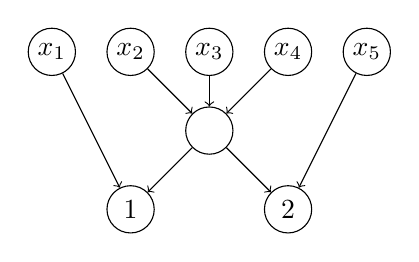
\begin{tikzpicture}
%\draw[help lines] (0,0) grid (10,6);
\foreach \x/\y/\n/\t in {0/4/x1/x_1, 1/4/x2/x_2, 2/4/x3/x_3, 3/4/x4/x_4, 4/4/x5/x_5, 2/3/a/~, 1/2/b/1, 3/2/c/2}
  \node[inner sep=0mm,circle,draw,minimum size=6mm] (\n) at (\x,\y) {$\t$};
\foreach \s/\t in {x2/a, x3/a, x4/a, a/b, x1/b, a/c, x5/c}
  \draw[->] (\s) -- (\t);
\end{tikzpicture}
\end{center}

A~{\em binary circuit} is a~circuit having no gates of fan-in more than two. It is not difficult to see that any circuit can be converted into a~binary circuit of size at most twice the size of the original circuit. For this, one just replaces every gate of fan-in~$k$, for $k>2$, by a~binary tree with $2k-2$ wires (such a~tree contains $k$~leaves hence $k-1$ inner nodes and $2k-2$ edges).

Clearly, in the binary circuit the number of gates does not exceed its size (i.e., the number of wires). And the number of gates in a~binary circuit is exactly the minimum number of semigroup operations needed to compute the corresponding function.

In a~special case of the Boolean semigroup $(\{0,1\}, \lor)$, such circuits are known as {\em rectifier networks}. An overview of known lower and upper bounds for such circuits is given by Jukna in \cite[Section~13.6]{DBLP:books/daglib/0028687}.




\section{Commutative Semigroups}
\todo[inline]{Vanya, go!}

We start with an almost trivial special case.

\begin{lemma}
Let $S$~be {\em any} semigroup (not necessarily commutative) and let $A \in \{0,1\}^{n \times n}$ contain at most one zero in every row. Then $C(Ax) \le O(n)$.
\end{lemma}
\begin{proof}
We first precompute all prefixes and suffixes of $x_1, \dotsc, x_n$. Namely, let $p_i=x_1x_2\dotsb x_i$. All $p_i$'s can be computed in $(n-1)$ binary gates as follows:
\[p_1=x_1, p_2=p_1x_2, p_3=p_2x_3, \dotsc, p_i=p_{i-1}x_i, \dotsc, p_n=p_{n-1}x_n \, .\]
Similarly, in $(n-1)$ binary gates we compute all suffixes $s_j$ (for all $1 \le j \le n$) where $s_j=x_jx_{j+1}\dotsc x_n$. From these prefixes and suffixes all the outputs can be computed as follows: if a~row of~$A$ contains no zeros, the corresponding output is~$p_n$; if a~row contains a~zero in position~$i$, the output is $p_{i-1}s_{i+1}$ (for $i=1$ and $i=n$ we just omit the redundant term).
\end{proof}



\subsection{Matrices with Constant Maximum Number of Zeros in Each Row}

\subsection{Matrices with Constant Average Number of Zeros in Each Row}

\section{Non-commutative Semigroups}
In the previous section, we have shown that for commutative semigroups dense linear operators can be computed by linear size circuits. A~closer look at the circuit constructions reveals that we use commutativity crucially: it is important that we may reorder the columns of the matrix. In this section, we show that this trick is unavoidable: for non-commutative semigroups, it is not possible to construct linear size circuits for dense linear operators. We do this by showing that, in the non-commutative case, the dense linear operator problem has linear size circuits iff the range queries problem has linear size circuits. We then use a~lower bound $\Omega(n\alpha(n))$ for the latter problem (over faithful semigroups) by Chazelle and Rosenberg~\cite{DBLP:journals/ijcga/ChazelleR91}. 

The equivalence between two problems is not difficult to prove for free semigroups. To make it more interesting, we prove the equivalence for idempotent semigroups. Hence, {\em throughout the whole section we assume that the semigroup under consideration is idempotent and faithful.}

\begin{theorem}
There exists dense matrices~$A$ such that $Ax$ cannot be computed by linear size circuits.
\end{theorem}

\begin{center}
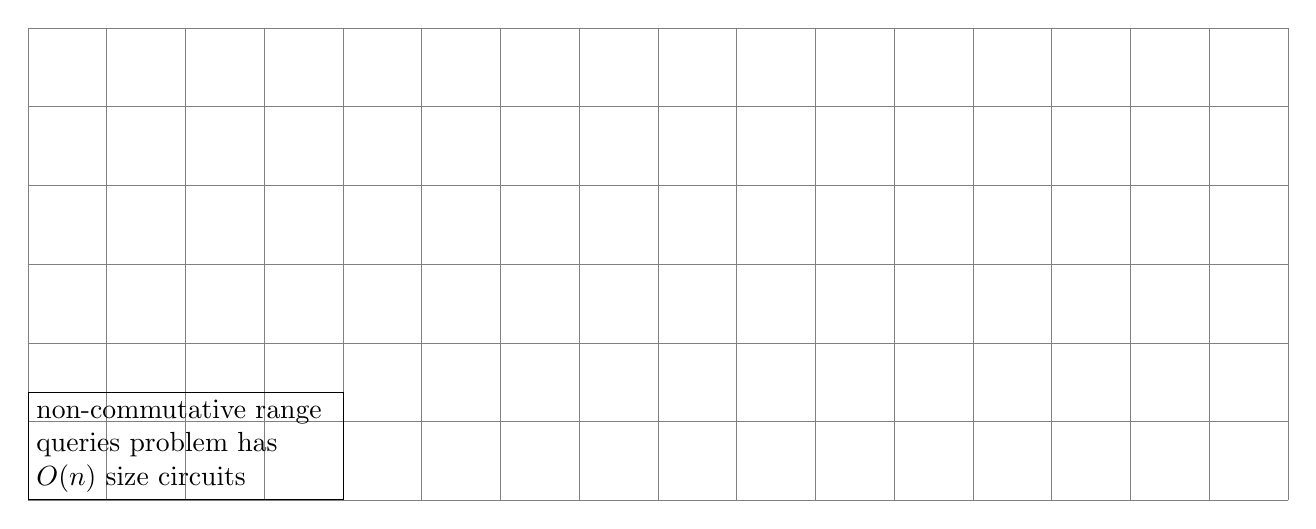
\begin{tikzpicture}
\draw[help lines] (0,0) grid (16,6);
\tikzstyle{v}=[rectangle,draw,inner sep=1mm,text width=38mm,above right]

\node[v] at (0,0) {non-commutative range queries problem has $O(n)$ size circuits};
\end{tikzpicture}
\end{center}



\begin{theorem}
Intervals are computable by $O(n)$-size circuit iff non-commutative dense matrices are computable by $O(n)$-size circuit.
\end{theorem}

To show the theorem we introduce an intermediate problem: computing non-commutative intervals by $O(n)$-size circuit.

Clearly, this problem subsumes both of our problems. Indeed, if we can compute non-commutative intervals, we can compute commutative intervals by the same circuit.
On the other hand, if we can compute non-commutative intervals, then given non-commutative dense matrix we can split it into intervals, compute them separately, then join them together in $O(n)$.

Thus, it remains to show the following two lemmas.

\begin{lemma} \label{lem:dense_matrices}
If we can compute non-commutative dense matrices by a linear size circuit, we can also compute non-commutative intervals.
\end{lemma}

\begin{lemma} \label{lem:intervals}
If we can compute commutative intervals by a linear size circuit, we can also compute non-commutative intervals.
\end{lemma}

\section{Proof of Lemma~\ref{lem:dense_matrices}}

The intuition why this might be true is that it seems that the best way to compute rows of dense matrix is to construct clauses with the correct order of variables. If this is true, then the idea is that we can extend each interval by variables on both sides (with small gaps on each side of the interval), thus obtaining a dense matrix. Then we can try to extract the computation of the intervals from the computation of the dense matrix. Since all rows of the matrix are hopefully computed by consecutively adding the variables in the correct order, we might be able to do that.

But some analysis of all these things is needed since idempotency is tricky. For example, it is possible to simulate commutativity: if we have the product $xy$ and would like to have $yx$ we can just multiply by $x$ from the left and by $y$ from the right. Then we have $xyxy=xy$. We can use this to put some variables inside of already produced products. If we have $xz$ and would like to obtain $xyz$ we can just multiply by $xyz$ from the left and by $xyz$ from the right. Then we have
$$
(xyz)xz(xyz)=xy(zxzx)yz=xy(zx)yz=xyz.
$$
This is not extremely impressive, since to obtain $xyz$ we multiply by $xyz$, but the point is that this is possible in principle. So, to prove the lemma some more work is needed.


So, we consider the free idempotent semigroup with generators $\{a_1,\ldots, a_n\}$.
We consider the generators to be ordered from $a_1$ to $a_n$ in the increasing order. We want to compute $B \cdot \vec{a}$, where $\vec{a}=(a_1,\ldots, a_n)$ and $B$ is a boolean matrix.

We will show that any circuit computing $B \cdot \vec{a}$ can be reconstructed into another circuit that we will call \emph{an interval circuit} without increase in the size of the circuit. In this circuit we require that each gate computes a word that is equivalent to a word consisting of increasing sequence of letters. Note that as a consequence we have that if in an interval circuit we multiply two gates $f$ and $h$, then the increasing sequences of letters computed by $f$ and $h$ are matching, that is some suffix of $f$ is equal to some suffix of $h$. Otherwise, the product is not equal to an increasing sequence of variables.

Once we show that any circuit solving our problem can be reconstructed into an interval one, it is easy to reduce an interval problem to our problem. Note, that given a circuit computing $B \cdot \vec{a}$ for a super-dense matrix $B$ we can construct a circuit computing all intervals of this matrix. Indeed, first reconstruct a circuit into an interval one. Then, once the interval circuit is trying to multiply intervals that have gaps  between them, we just not multiply them. Later on if we try to do something with the product we have not computed we use the left of its inputs in case we try to multiply from the left, and the right input if we are multiplying from the right. So, if we need to solve an interval problem, for each interval we skip one variable on each side and add all other variables to the interval. This turn our problem into the super-dense matrix. We compute this matrix, then deduce the computation of intervals as described above.

%For each gate $g$ of the circuit we will consider the word $W_g$ computed in this gate. This word is defined recursively as a concatenation of the words corresponding to input gates. For each gate $g$ we say that the letter $a$ is \emph{good} in $W_g$ if $a$ is present in $W_g$ and $W_g$ will not be multiplied on the left by words containing larger or equal letters then $a$.

To reconstruct a circuit into a linear one we need to introduce some notation. Consider a circuit $C$ and its gate $g$.
We will identify gates and words that they are computing. We will treat the results of the computation of the gates as words to which gates apply concatenation operation. That is, we consider these words before we apply any equivalences in the semigroup to them.
Suppose letter $a_i$ is contained in $g$. We say that $a_i$ is \emph{good} in $g$ if there is a path in $C$ from $g$ to some output, on which the word is never multiplied from the left by words with letters greater or equal to $a_i$.

Note that if $a_i$ and $a_{i'}$ are contained in $g$, $i<i'$ and $a_i$ is good in $g$, then $a_{i'}$ is also good in $g$. That is, the set of all good letters in $g$ is closed upwards.

Consider the largest good letter in $g$ (if there is one), denote it by $a_k$ (if there are good letters in $g$, then $a_k$ is actually just the largest letter in $g$). Consider the first occurrence of $a_k$ in $g$.

\begin{claim}
All first occurrences of other good letters in $g$ must be to the left of $a_k$.
\end{claim}

\begin{proof}
Suppose that some good letter $a_i$ has the first occurrence to the right of $a_k$. Consider an output $c$ such that there is a path from $g$ to $c$ and along this path there are no multiplications of $g$ from the left by words containing letters greater than $a_i$. Then we have $c \sim LgR$, where all letters of $L$ are smaller then $a_i$. Then in $c$ letter $a_i$ appears before $a_k$ when we read from left to right, and in $RgL$ we have that $a_k$ appears before $a_i$. This contradicts Lemma~\ref{lem:variables_order}.
\end{proof}

Consider for the gate $g$ two words, $\mmin_g$ and $\mmax_g$. Both this words are products of variables in the increasing order: $\mmin_g$ is the product of good letters of $g$ in the increasing order, $\mmax_g$ is the product (in the increasing order) of all letters that has first occurrences before $a_k$. Note that $\mmin_g$ is a suffix of $\mmax_g$. If there are no good letters in $g$ we just let $\mmin_g=\mmax_g=\lambda$ (the empty word).

For the word $W$ that has the form of the product of variables in the increasing order we call $a_j$ a \emph{gap variable} if it is not contained in $W$ and there are $a_i$ and $a_l$ contained in $W$ such that $i<j<l$.

We will show how given a circuit $C$ to construct an interval circuit $C'$ that for each gate $g$ of $C$ computes some intermediate product $P_g$ between $\mmin_g$ and $\mmax_g$: we will have that $\mmin_g$ is a suffix of $P_g$ and $P_g$ is a suffix of $\mmax_g$. The size of $C'$ is at most the size of $C$.
Note that for an output gate $g$ we have $\mmin_g=\mmax_g=g$, so the circuit $C'$ computes the correct outputs.

The construction of $C'$ is by induction on the number of gate. For the case of input gate $g$ everything is obvious: $\mmax_g$ is either $\lambda$, or $a_j$ for some variable $a_j$. Both of these are easy to compute.

For the step of induction consider a gate $g=f\cdot h$ computed as a product of two previous gates.

Consider the good letters in $g$. If there are none, we can just let $P_g=\lambda$ and there is no computation needed.

If all first occurrences of good letters of $g$ are lying in one of the input gates $f$ and $h$, then they are good in the corresponding input gate. So we can set $P_g$ to $P_f$ or $P_h$ and there is no computation needed.

The only remaining case is that some good letters have their first occurrence in $f$ and some in $h$. Then the largest letter $a_k$ of $g$ has the first occurrence in $h$ and all letters of $f$ are smaller than $a_k$.

\begin{claim} \label{cl: h is good}
There are no gap letters for $\mmax_h$ in $f$.
\end{claim}

\begin{proof}
Suppose that some letter $a_i$ in $f$ is a gap letter for $\mmax_h$. Consider an output $c$ such that there is a path from $g$ to $c$ and along this path there are no multiplications of $g$ from the left by words containing letters greater than $a_k$. Then we have $c \sim LgR$, where all letters of $L$ are smaller then $a_k$. Consider the prefix $P$ of $c$ preceding the letter $a_k$ and the prefix $Q$ of $Lg$ preceding the letter $a_k$.
Then by Lemma~\ref{lem:prefix_equivalence} we have $P \sim Q$. But then the letters of $P$ and $Q$ appear in the same order if we read the words from right to left. But this is not true (the letters in $P$ are in the decreasing order and in $Q$ the letter $a_i$ is not on its place), so we get a contradiction.
\end{proof}

\begin{claim}\label{cl: f is good}
There are no gap letters for $\mmax_f$ in $h$.
\end{claim}

\begin{proof}
Suppose that some letter $a_i$ in $h$ is a gap letter for $\mmax_f$. Consider an output $c$ such that there is a path from $g$ to $c$ and along this path there are no multiplications of $g$ from the left by words containing letters greater than $a_l$, the largest letter of $f$. Then we have $c \sim LgR$, where all letters of $L$ are smaller then $a_l$. Consider the prefix $P$ of $c$ preceding the letter $a_l$ and the prefix $Q$ of $Lg$ preceding the letter $a_l$.
Then by Lemma~\ref{lem:prefix_equivalence} we have $P \sim Q$. But then the letters of $P$ and $Q$ appear in the same order if we read the words from right to left. But this is not true(the letters in $P$ are in the decreasing order and in $Q$ the letter $a_i$ is not on its place), so we get a contradiction.
\end{proof}

Consider $P_f$ and $P_h$. From two Claims~\ref{cl: h is good} and~\ref{cl: f is good} we know that they are intervals in the same sequence of variables $\var(P_f)\cup \var(P_h)$. We know that the largest letter of $P_h$ is greater than all letters of $P_f$. Then either $P_f$ is contained in $P_h$, and then we can let $P_g=P_h$ (it contains all good letters of $g$), or we have $P_f =PQ$ and $P_h=QR$ for some words $P, Q, R$. In the latter case we can let $P_g = P_f \cdot P_h = PQQR=PQR$. Clearly, $\mmin_g$ is the suffix of $P_g$ and $P_g$ itself is the suffix of $\mmax_g$. So, we are done.




\section{Proof of Lemma~\ref{lem:intervals}}

For the proof of this lemma we will show that any computation of commutative intervals can be reconstructed without increase in the number of gates in such a way that each gate computes an interval (still commutatively; let's call this an interval circuit). It is easy to see that then this circuit can be reconstructed as a non-commutative circuit each gate of which computes the same interval with the variables in the right order. Indeed, we need to make sure that each gate computes an interval in such a way that all variables are in the right order and this is easy to do by induction. Each gate computes an OR of two intervals $a$ and $b$. If one of them is contained in the other, we simplify the circuit, since the gate just computes the same interval as one of its inputs. It is impossible that $a$ and $b$ are non-intersecting and have a gap between them, since then our gate does not compute an interval (in the interval circuit). So, if $a$ and  $b$ are non-intersecting, then they are consecutive and we just need to multiply then in the right order. If the intervals are intersecting, we just multiply then in the right order and apply idempotency (like this: $(x_1x_2x_3)(x_2x_3x_4)=x_1(x_2x_3)(x_2x_3)x_4=x_1x_2x_3x_4$).

Thus it remains to show that each non-commutative circuit can be reconstructed into an interval circuit. For this we will need some notation.

Suppose we have some circuit $C$. For each gate $g$ denote by $\lef(g)$ the smallest index of the variable in $g$ (the leftmost variable). Analogously denote by $\righ(g)$ the largest index of the variable in $g$. Denote by $\gap(g)$ the smallest $i$ such that $x_i$ is not in $g$, but there are some $j,k$ such that $j<i<k$ and $x_j$ and $x_k$ (the smallest index of the variable that is in the gap in $g$).
%If there is no such variable (that is, $g$ computes an interval), then $\gap(g)=n+1$.
Next, fix some ordering of gates in $C$ (the ordering should be proper, that is inputs to any gate should have smaller numbers). Denote by $\num(g)$ the number of a gate in this ordering. Finally, by $\out(g)$ denote the out-degree of $g$.

For each gate that computes a non-interval consider the tuple
$$
\tup(g)=(\lef(g),\gap(g),\num(g),-\out(g)).
$$ For the circuit $C$ consider $\tup(C) = \min_g \tup(g)$, where the minimum is considered in the lexicographic order and is taken over all non-interval gates. If there are no non-interval gates we let $\tup(C)=\infty$. This is our semi-invariant, we will show that if we have a circuits that is not an interval circuit, we can reconstruct it to increase  its $\tup$ (in the lexicographic order) without increasing its size. Since $\tup$ ranges over a finite set, we can reconstruct the circuit repeatedly and end up with an interval circuit.

Now we are ready to describe a reconstruction. Consider a circuit $C$ that is not an interval circuit. And consider a gate $g$ such that $\tup(g)=\tup(C)$ (it is clearly unique). Denote by $a$ and $b$ two inputs of $g$. Let $i=\lef(g)$ and $j=\gap(g)$, that is $x_i$ is the variable with the smallest index in $g$ and $x_j$ is the first gap variable of $g$ (it is not contained in $g$).

The variable $x_i$ is contained in at least one of $a$ and $b$. Consider the gate among $a$ and $b$ that contains $x_i$. It also contain all variables between $x_i$ and $x_j$ (but not $x_j$), since the converse would contradict minimality of $g$ (by the second coordinate of $\tup$). But this gate cannot have $x_j$ as a gap variable: it would also contradict minimality of $g$ (by the third coordinate of $\gap$). Thus this gate is exactly the interval $[x_i,x_j)$ (by this we denote the product of variables from $x_i$ to $x_j$ excluding $x_j$). In particular, only one of $a$ and $b$ contains $x_i$: otherwise they are both $[x_i,x_j)$ and $x_j$ is not a gap variable for $g$.

From now on we assume that $a$ contains $x_i$, that is $a=[x_i,x_j)$.
%Note that then $b$ contains all variables to the right of $x_j$, in particular the variable with the largest index in $g$.

Now we consider all gates $h_1,\ldots, h_k$ that have edges leading from $g$. Denote by $f_1,\ldots, f_k$ their other inputs. If $k$ is equal to $0$, we can remove $g$ and reduce the circuit. Now we consider cases.

Case 1. Suppose that there is $l$ such that $\lef(f_l) \leq \lef(g)$. Then $f_l$ contains all variables in $[x_i,x_j)$ (the contrapositive contradicts the minimality of $g$ by the second coordinate of $\gap$). Thus $f_l$ contains $a$. Then, we can restructure the circuit by feeding $b$ to $h_l$ instead of $g$. This does not change the clause computed by $h_l$ and reduces $\out(g)$. Thus $\tup(C)$ increases and we are done.

Case 2. Suppose that for all $l$ we have $\lef(f_l)>\lef(g)$. Consider $l$ such that $f_l$ has the minimal $\righ(f_l)$ (if there are several such $l$ pick among them the one with the minimal $\num(f_l)$). Now we restructure the circuit in the following way. We feed $f_l$ to $g$ instead of $a$. We feed $a$ to $h_l$ instead of $f_l$. We feed $h_l$ to all other $h_p$'s instead of $g$. It is not hard to see that all these reconstructions are valid, that is, do not create cycles. Note that they might require reordering of the circuit gates, since we create edges between previously incomparable $h$-gates. But the reording changes only for the gates with $\num$ greater than $\num(g)$.

Observe, that the circuit still computes the outputs correctly. The changes are in the gates $h_1\ldots, h_k$ (and also in $g$, but $h_1,\ldots, h_k$ are all of its outputs). $h_l$ does not change. Other $h_p$'s might have changed, they now additionally include variables of $f_l$. But note that all of these variables are in between of $\lef(h_p)$ and $\righ(h_p)$, so they must be presented in the output gates connected to $h_p$ anyway.

Now, observe that $\num(g)$ has increased (by the first coordinate). There are no new gates with smaller $\lef$. Among gates with the minimal $\lef$ there are no new gates with smaller $\gap$. Among gates with minimal $(\lef,\gap)$ all gates have larger $\num$ then $g$. Thus $\tup(C)$ increased and we are done.

\section{Applications}
\todo[inline]{Andrey, go!}

\bibliographystyle{plain}
\bibliography{text}

\end{document}